\chapter{Background}
In questo capitolo verrà descritta la tecnologia alla base di Bitcoin. Particolare attenzione verrà data alla blockchain, la struttura dati che costituisce il libro contabile, al funzionamento delle transazioni, agli indirizzi per introdurre infine la questione relativa all'anonimato. 
%1- Spiegare cosa sono i btcoin("storia" ecc...)
%2- Spiegare la blockchain(definizione)
%3- Spiegare address, wallet(anonimato), generazione indirizzi
%4- concentrarsi sulle transazioni(differenza teoria e pratica anonimato), come avvengono come funzionano %la fee ecc...
%Ricorda di mettere immagini
\section{Bitcoin}
Bitcoin, l’unità monetaria elettronica a cui facciamo riferimento in questa tesi, è stata sviluppata da Satoshi Nakamoto, un misterioso autore giapponese la cui identità resta a tutt'oggi ignota, tanto da indurre molti a pensare che si tratti di uno pseudonimo, o che dietro a tale nome si celi in realtà non una singola persona, ma addirittura un gruppo di ricercatori o di informatici. L’articolo in cui viene presentato l’intero protocollo Bitcoin viene pubblicato nel 2008, sotto il nome di ”Bitcoin: A Peer-to-Peer Electronic Cash System”\cite{nakamoto2009bitcoin}; il paper è facilmente reperibile e contiene la descrizione dettagliata del protocollo alla base del funzionamento di Bitcoin.\\La peculiarità di tale sistema è l’uso di una rete secondo il modello Peer-to-Peer per effettuare, diffondere e validare le transazioni, e l’intero storico di esse viene mantenuto in un libro contabile distribuito e di pubblica consultazione. La grande e difficile sfida che Bitcoin dunque si pone è quella di coniugare l’anonimato degli utenti con un’alta affidabilità relativamente alle transazioni e alla loro validità e integrità.\\A fronte della sfida di trasparenza versus affidabilità, è fondamentale definire un’implementazione del libro contabile che impedisca alterazioni di transazioni già registrate e validate: ricordiamo che in questo contesto paritario e distribuito, nessun controllo viene effettuato da parte di entità centrali, come per esempio le banche.\\
La soluzione ideata da Nakamoto per garantire l’integrità dello storico delle transazioni è stata quella di implementare il libro contabile tramite una particolare struttura dati: la blockchain.\\Come suggerisce il nome, la struttura si compone di una serie di blocchi collegati tra di loro come in una catena: ogni blocco racchiude un insieme di transazioni effettuate in un certo periodo temporale.\\Il blocco corrente, non ancora inserito, contiene le ultime transazioni la cui legittimazione deve essere ancora approvata, mentre i blocchi precedenti, già
agganciati alla catena, si riferiscono a transazioni già validate, e la blockchain è fin lì immutabile. Il meccanismo che garantisce la totale immutabilità della struttura, pena la sua completa invalidazione, è la crittografia.\\\\
\begin{figure}[h!]
    \centering
    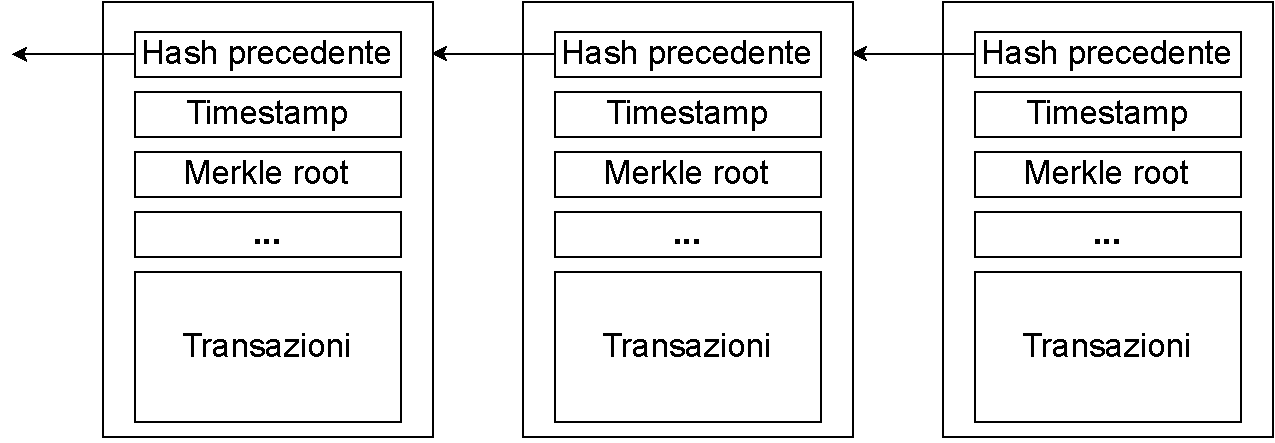
\includegraphics[scale=0.6]{Images/blockChaining.pdf}
    \caption{Schema della Blockchain}
    \label{fig:blockchain}
\end{figure}
\FloatBarrier
\section{Blockchain}
Un generico blocco Bi all’interno della blockchain contiene la sequenza di transazioni relative ad un certo periodo temporale (supponiamo che siano n: T1 , T2 , ... ,Tn ) e un valore hash $h_{i-1}$ identificativo del blocco precedente nella catena, che è l’output di una funzione hash crittografica (la cui definizione sarà data nel seguito).\\È inoltre presente un campo detto nonce, che servirà per l’operazione di mining, ovvero il procedimento che porta all’aggiunta di un nuovo blocco alla blockchain. Sono presenti anche altri dati all’interno del blocco, ma al fine di descrivere il meccanismo crittografico che salvaguarda l’integrità della struttura questo livello di dettaglio è sufficiente.\\\\\\In Figura \ref{fig:blocchi} è rappresentata la struttura di un generico blocco Bi all’interno della blockchain.
\begin{figure}[h!]
    \centering
    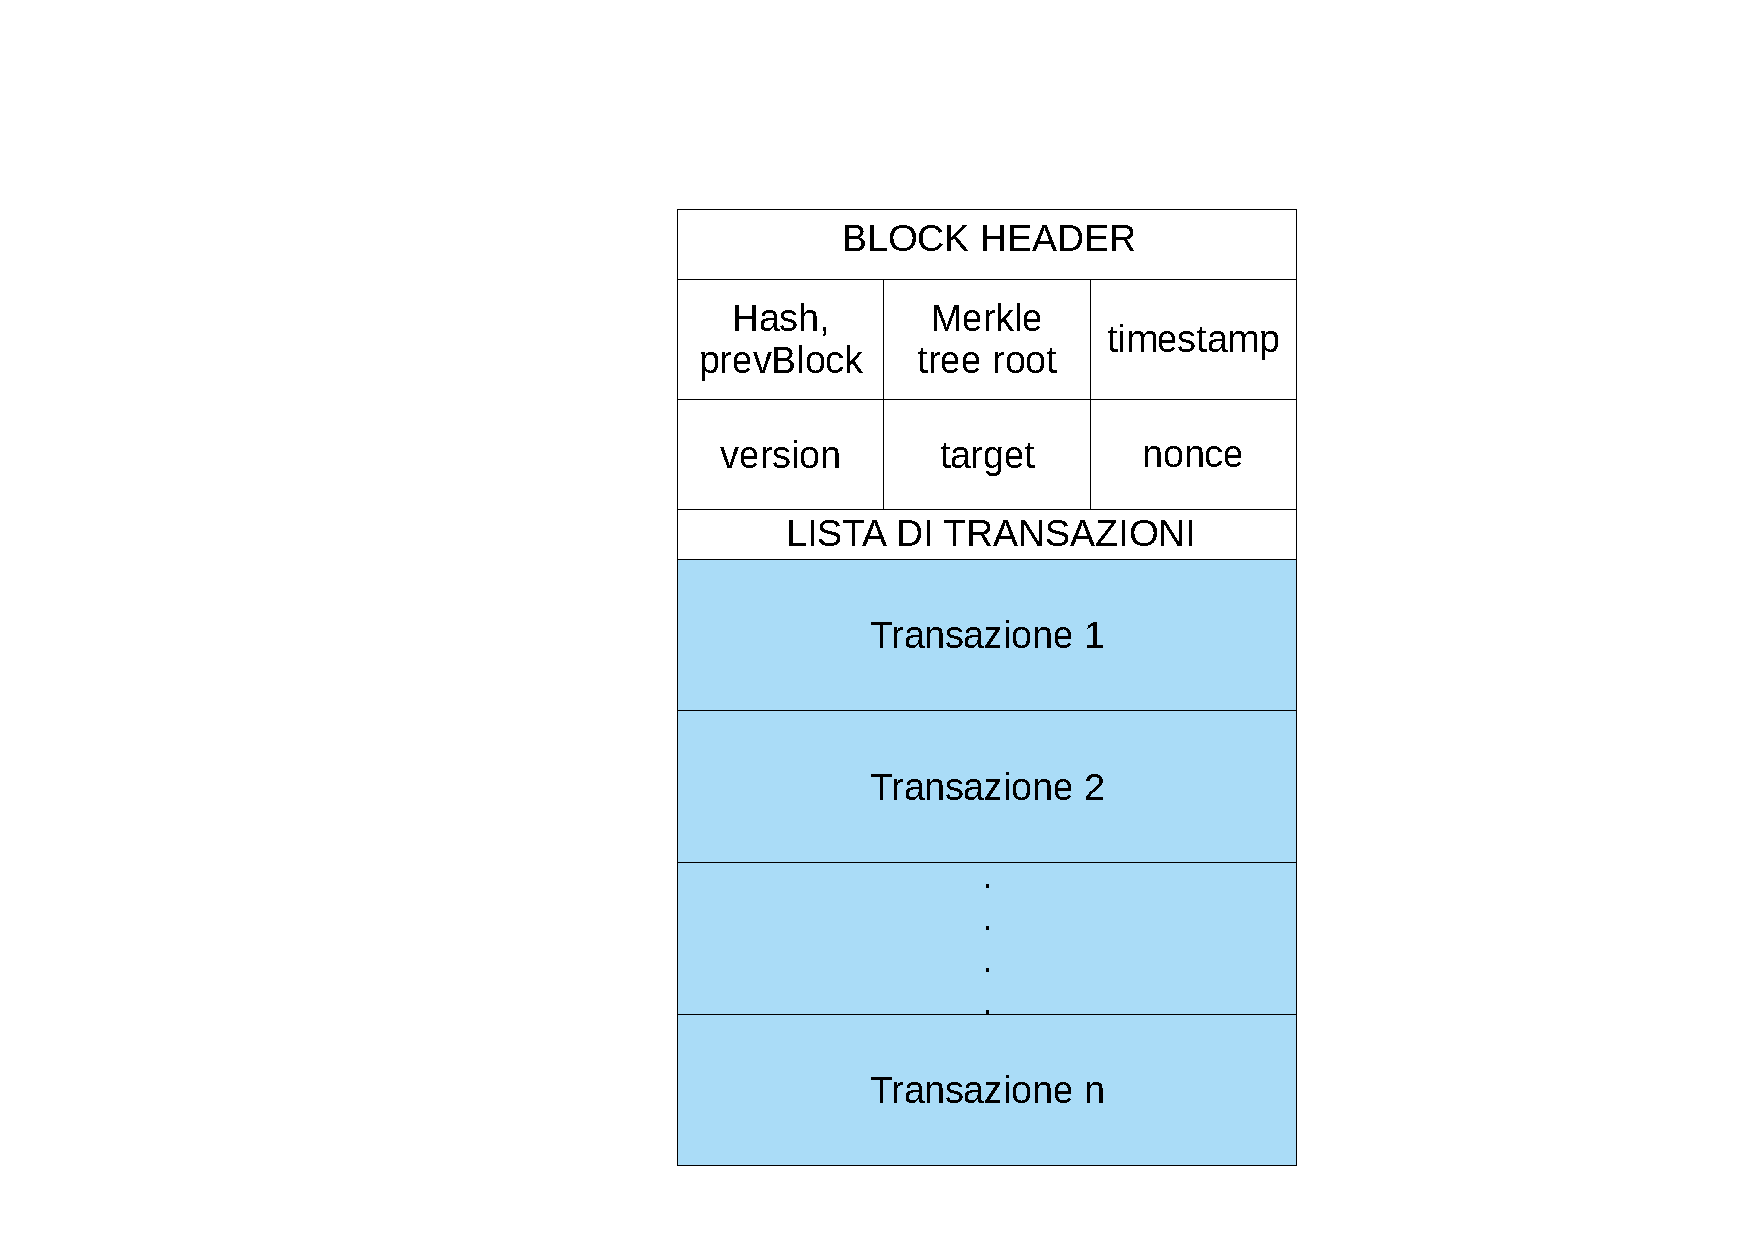
\includegraphics[scale=0.4, trim = 0cm 0cm 0cm 3cm, clip]{Images/blocco_singolo.pdf}
    \caption{Schema di un generico blocco}
    \label{fig:blocchi}
\end{figure}
\FloatBarrier
Come accennato sopra, ogni blocco ha un suo identificativo univoco, una sor-
ta di impronta digitale personale, che è l’output di una opportuna funzione
hash.\\
Una funzione hash $f$: X $\longrightarrow$ Y è una funzione matematica avente come dominio X e codominio Y, insiemi finiti tali che $|X| >> |Y |$.\\Tale funzione prende in input elementi di X di lunghezza qualsiasi e produce in output, a prescindere dalla lunghezza dell’input, stringhe binarie di dimensione fissa, i cosiddetti fingerprint, chiamati anche immagini hash o semplicemente hash.\\
Una proprietà fondamentale delle funzioni hash è relativa al tempo necessario al loro calcolo: devono essere calcolate efficientemente, ossia a fronte di un input di $m$ bit, la complessità computazionale per produrne il fingerprint deve essere $O(m)$, lineare o comunque polinomiale nei bit su cui è rappresentato l’input.\\ Vista la grande differenza di cardinalità tra i due insiemi X e Y, inevitabilmente alcuni input diversi della funzione hash avranno la stessa immagine; questo fenomeno è detto collisione: $x_1$ e $x_2$ $\in$ X, con $x_1 \neq x2$ , collidono se la loro immagine hash è la stessa ( f ($x_1$ ) = f ($x_2$ ) ).\\In crittografia si usano alcune famiglie di funzioni hash molto particolari, dette funzioni hash one-way o funzioni hash crittografiche, le quali devono rispettare altre importanti proprietà oltre a quelle descritte sopra:
\begin{enumerate}
    \item \textbf{Proprietà di one-way}: dato y $\in$ Y, output della funzione f, deve essere computazionalmente difficile invertire la funzione, ossia trovare un x $\in$ X tale che f (x) = y. Il termine one-way significa proprio questo: una funzione hash ”facile” da calcolare (complessità polinomiale nel numero di bit dell’input) ma ”difficile” da invertire (complessità esponenziale, il che rende l’inversione inattuabile all’atto pratico).
    \item \textbf{Proprietà di claw-free}: Per la funzione f , deve essere computazionalmente difficile determinare due elementi $x_1$ e $x_2 \in$ X ($x_1 \neq x_2$) tali che f ($x_1$ ) = f ($x_2$). Ciò significa che per una funzione hash crittografica non deve essere possibile trovare due elementi che collidono in tempo ragionevole.
\end{enumerate}
Un insieme di funzioni hash crittografiche ampiamente usate è quello delle SHA (Secure Hash Algorithm). Una di queste è la SHA-256, funzione hash crittografica che da input di dimensioni variabili produce un fingerprint della lunghezza fissa di 256 bit, ed è la funzione utilizzata per calcolare gli hash dei blocchi all’interno della blockchain.\\L’immagine hash del blocco $B_i$ è calcolata applicando la SHA-256 all’input formato dalla concatenazione delle transazioni lì contenute con il nonce e l’hash del blocco precedente, come riassunto dalla seguente formula (H è una funzione hash crittografica, in genere la SHA-256, e il simbolo $||$ è l’operatore di concatenazione):
\begin{center}
    $hash(B_i) = H(T_1||T_2||...||T_n||hash(B_{i-1})||nonce)$
\end{center}
\begin{figure}[h!]
    \centering
    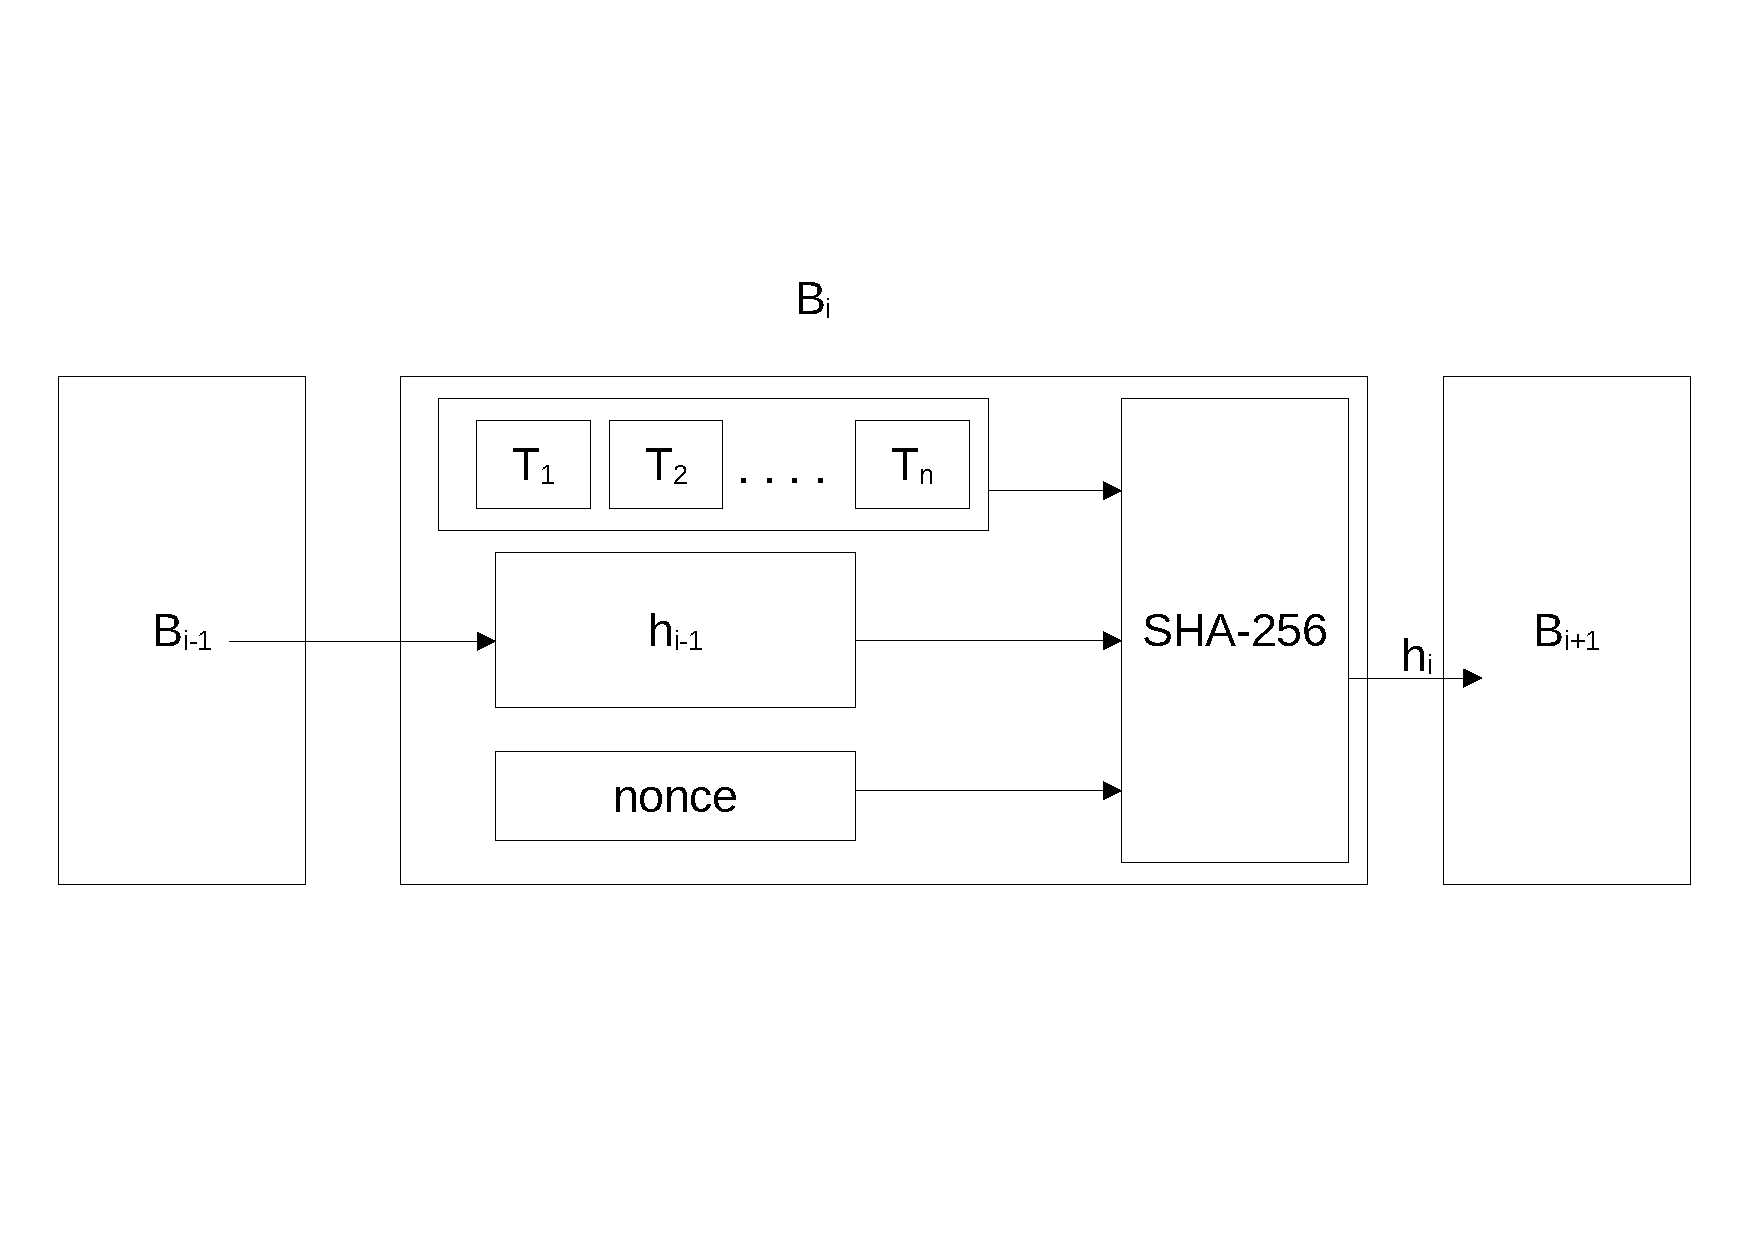
\includegraphics[scale=0.5, trim = 1cm 4cm 0cm 4cm, clip]{Images/blocchi_sha.pdf}
    \caption{Calcolo hash blocco $B_i$}
    \label{fig:sha-256}
\end{figure}
\FloatBarrier
Mentre le transazioni, e quindi anche la loro concatenazione, sono note nel blocco, così come è noto l’hash proveniente dal blocco precedente, il valore del nonce è incognito. L’attività di mining consiste nel risolvere un puzzle crittografico: trovare il valore del nonce tale che l’immagine hash prodotta dalla SHA-256 inizi esattamente con $t$ zeri, dove $t$ è un valore prefissato dal sistema, e variabile nel tempo.\\
La ricerca del nonce per la corretta aggiunta di un blocca è denominata \textbf{Proof of work}. L'unico modo per di trovare il nonce che produca un fingerprint che inizi con $t$ zeri, è quello di applicare ripetutamente la funzione SHA-256 con nonce via via diversi, finchè non si giunge ad un hash che soddisfa la proprietà desiderata. La risoluzione del problema è esponenziale in $t$, infatti la ricerca del nonce richiede tempo $O(2^t)$, ciò rende il problema di difficile risoluzione, in quanto è necessario far eseguire una lunga serie di calcoli alle macchine; nella pratica i calcolatori sono stati ottimizzati a livello hardware con lo scopo di calcolare il più rapidamente possibile la funzione SHA-256. Il valore di t viene aggiornato periodicamente dal sistema, in modo che la validazione di un blocco richieda sempre in media circa 10/15 minuti di tempo.\\Questo sistema evita che i blocchi già inseriti possano essere modificati retroattivamente: cambiando il contenuto di un blocco, ne cambierebbe anche il valore hash, e ciò implica il dover ricalcolare tutti i nonce dei blocchi successivi ad esso, perchè altrimenti le immagini hash non corrisponderebbero più tra blocchi consecutivi; dunque ciò che è stato scritto sulla blockchain è da considerarsi immutabile, a meno di rendere inconsistente tutta la struttura anche alterandone una sola transazione.
\todo{dopo pranzo}finire discorso background


